\documentclass{article}
\usepackage[utf8, margin=1.3in, top=1in, bottom=1in]{geometry}
\usepackage{pdfpages}

\title{Usability test report (MVP)}
\author{Mikkel Aas \and Magnus Gluppe \and Jakob Frantzvåg Karlsmoen \and Mikael Falkenberg Krog}
\date{March 2020}


\begin{document}

\maketitle

\section{Introduction}
MetIma serves as an image gallery that allows the user to view the metadata of each image. We have conducted a usability test using the MVP. There were two participants; an observer and a participant. The observer captured the participants comments, navigational choices, task completion rate, comments, overall satisfaction rating, questions and feedback.

\subsection{Summary}
The most important findings were that our design was mostly intuitive, but a feature to import multiple images at the same time and prioritization of more relevant metadata would be good to include.


\subsection{Demographic}
For a demographic we wanted to include several different age groups. We therefore found four individuals to perform user testing on. One in their late 10's, one in their mid-20's and two in their early 50's. We felt this was a diverse age group, and would give valuable feedback to use in developing the application for most users.

\subsection{Tasks}
Since we now had our MVP working, we could almost test the application to it's full extent. While it was still very basic UI-wise, it had almost all functionality implemented and working enough to have it tested.
\section{Results}

\subsection{Usability Problems}
The main complaint among all testers were the missing ability to add several images at once. In the current state, both the UI and performance is not able to handle a huge amount of images. We expect this problem to be solved in the final product.

Another big complaint was that the metadata displayed for the images is not very useful to the average user. The metadata displayed is the raw metadata extracted from the image, and includes all data available. A possible solution to this is to only display the most relevant information (date, resolution, camera etc), and have an option to display the rest of the data.

\subsection{Other Feedback}
A lot of the feedback was directly on the usability and design of the application. Elements such as design of input boxes, no icons and small buttons are all problems that will be solved in the final product where we will have fully developed the UI to be like the wireframe.
\newpage

\section{MetIma Wireframe}
\begin{figure}[h]
   \centering
   \begin{tabular}{@{}c@{\hspace{.5cm}}c@{}}
       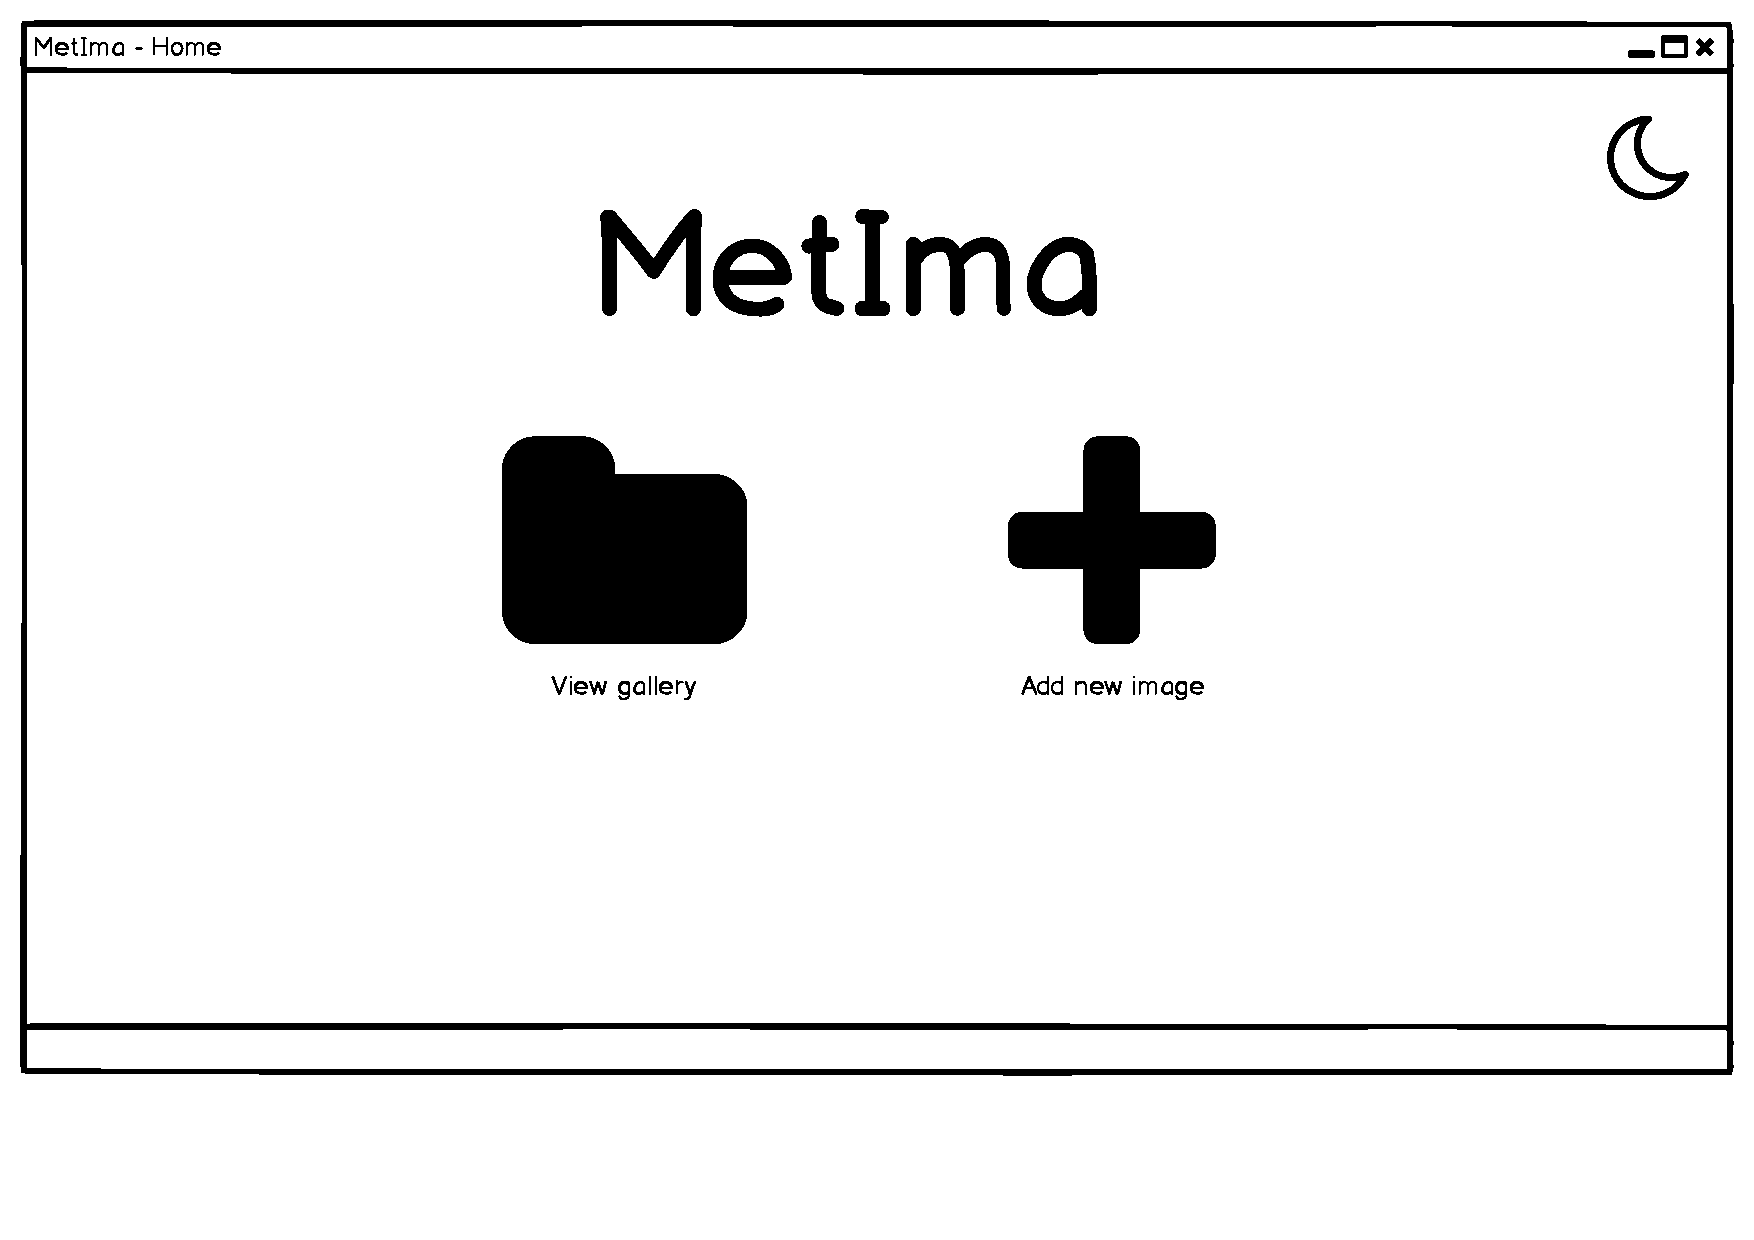
\includegraphics[page=1,width=.75\textwidth]{Wireframe SUP.pdf} \\[.5cm] 
       \includegraphics[page=2,width=.75\textwidth]{Wireframe SUP.pdf} \\[.5cm]
   \end{tabular}
\end{figure}
\begin{figure}[h]
   \centering
   \begin{tabular}{@{}c@{\hspace{.5cm}}c@{}}
       \includegraphics[page=3,width=.75\textwidth]{Wireframe SUP.pdf} \\[.5cm]
       \includegraphics[page=4, width=.70\textwidth]{Wireframe SUP.pdf}
   \end{tabular}
\end{figure}


\end{document}